
% This LaTeX was auto-generated from an M-file by MATLAB.
% To make changes, update the M-file and republish this document.

\documentclass{article}
\usepackage{graphicx}
\usepackage{color}
\usepackage{listings}
\usepackage[framed]{mcode}
\usepackage{fullpage}
\usepackage{hyperref}
\usepackage{amsmath}

\definecolor{lightgray}{gray}{0.5}
\setlength{\parindent}{0pt}

\begin{document}

    
    \begin{par}

\title{BE 521 - Homework 3\\{\normalsize Spring 2015}}
\author{Mike Lautman}
\date{\today}
\maketitle
\textbf{Objective:} Computational modeling of neurons.

\end{par}
\begin{lstlisting}
close all; clear all; clc;
\end{lstlisting}
\begin{par}

\section*{1.1a Basic Membrane and Equilibrium Potentials (5 pts)}

\end{par}
\begin{lstlisting}
time = 3;             % S
wave_f = 2;           % Hz
sample_f = 100;       % Hz

s= 0;
e = 2 * pi * wave_f * time;     % rad
steps = time * sample_f;

x = linspace(s, e, steps);
y = sin(x);

figure(1)
plot(x,y)
title('2 Hz sin Wave');
ylabel('Amplitude');
xlabel('time (S)')
\end{lstlisting}


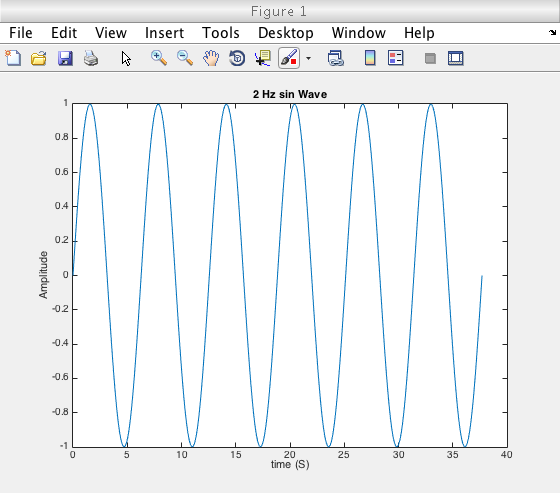
\includegraphics [width=4in]{BE521HW3_mlautman_01.png}
\begin{par}

\section*{1.1b Like length computation}

\end{par}
\begin{lstlisting}
LL = @(x) sum(abs(diff(x)));
\end{lstlisting}
\begin{par}

\section*{1.1c Like length of sign wave}

\end{par}
\begin{lstlisting}
lls = LL(y) % line lenght computation
\end{lstlisting}

\color{lightgray} \begin{lstlisting}
lls =

  23.984216311421108

\end{lstlisting} \color{black}
\begin{par}

\section*{1.2a Number of full windows}

\end{par}
\begin{lstlisting}
windows = @(xlen, fs, winLen, winDisp) (...
    ((xlen / fs) - winLen) / winDisp + 1 ...
);
\end{lstlisting}
\begin{par}

\section*{1.2b Windows in a sin wave}

\end{par}
\begin{lstlisting}
window_len = 0.5;    % S
win_disp = 0.25;      % S
windows_s = windows(length(x), sample_f, window_len, win_disp)
\end{lstlisting}

\color{lightgray} \begin{lstlisting}
windows_s =

    11

\end{lstlisting} \color{black}
\begin{par}

\section*{1.2c Windows in a sin wave. 500ms displacement}

\end{par}
\begin{lstlisting}
win_disp = .5;      % s
windows_s = windows(length(x), sample_f, window_len, win_disp)
\end{lstlisting}

\color{lightgray} \begin{lstlisting}
windows_s =

     6

\end{lstlisting} \color{black}
\begin{par}

\section*{1.2c Windows in a sin wave. 100ms displacement}

\end{par}
\begin{lstlisting}
win_disp = .1;      % s
windows_s = windows(length(x), sample_f, window_len, win_disp)
\end{lstlisting}

\color{lightgray} \begin{lstlisting}
windows_s =

    26

\end{lstlisting} \color{black}
\begin{par}

\section*{1.3a Moving Win Features}
\lstinputlisting{../MovingWinFeats.m}

\end{par}
\begin{par}

\section*{1.3b Windowed LL from 1.1}

\end{par}
\begin{lstlisting}
win_len = .5;
win_d = .25;
moving_LL = MovingWinFeats(y, sample_f, win_len, win_d, LL )
\end{lstlisting}

\color{lightgray} \begin{lstlisting}
moving_LL =

   3.889549524421202
   3.891483740328599
   3.892988351961849
   3.894063193217832
   3.894708145438365
   3.894923137423294
   3.894708145438366
   3.894063193217838
   3.892988351961849
   3.891483740328595
   3.889549524421203

\end{lstlisting} \color{black}
\begin{par}

\section*{1.3c}

\end{par}
\begin{lstlisting}
time = 3;
sample_f = 100;
steps = time * sample_f;

wave_f_1 = 2;
wave_f_2 = 5;

s = 0;
e1 = 2 * pi * wave_f_1 * time;
e2 = 2 * pi * wave_f_2 * time;

x1 = linspace(s,e1,steps);
x2 = linspace(s,e2,steps);

y1 = sin(x1);
y2 = sin(x2);

y = y1 + y2;

win_len = .5;
win_d = .25;

moving_LL = MovingWinFeats(y, sample_f, win_len, win_d, LL)
\end{lstlisting}

\color{lightgray} \begin{lstlisting}
moving_LL =

  10.215693178229969
  11.541338604412854
  10.035631811767006
   8.972801954378578
  10.126639055919377
  11.568020746303253
  10.126639055919368
   8.972801954378589
  10.035631811767008
  11.541338604412838
  10.215693178229980

\end{lstlisting} \color{black}
\begin{par}

\section*{1.4a area}

\end{par}
\begin{lstlisting}
area = @(x) sum(abs(x));
\end{lstlisting}
\begin{par}

\section*{1.4b energy}

\end{par}
\begin{lstlisting}
energy = @(x) sum(x.^2);
\end{lstlisting}
\begin{par}

\section*{1.4c Zero-crossings }

\end{par}
\begin{lstlisting}
z_crossings = @(x) sum(abs(diff(sign(x-mean(x)))))/2;
\end{lstlisting}
\begin{par}

\section*{1.4d All 4 with right allignment}

\end{par}
\begin{lstlisting}
win_len = .5;
win_d = .1;

y_a = MovingWinFeats(y, sample_f, win_len, win_d, area);
y_eng = MovingWinFeats(y, sample_f, win_len, win_d, energy);
y_x = MovingWinFeats(y, sample_f, win_len, win_d, z_crossings);
y_LL = MovingWinFeats(y, sample_f, win_len, win_d, LL);
y_nwindows = windows(length(y), sample_f, win_len, win_d);

x =linspace(win_len, time, y_nwindows);

figure(2)

subplot(3,2,1)
plot(x, y_LL);
title('Line Lenght')
xlabel('Time (s)')
ylabel('Line length (Units)')

subplot(3,2,2)
plot(x, y_a);
title('Area')
xlabel('Time (s)')
ylabel('Area (Units)')

subplot(3,2,3)
plot(x, y_eng);
title('Energy')
xlabel('Time (s)')
ylabel('energy (Units)')

subplot(3,2,4)
plot(x, y_x);
title('Mean Crossings')
xlabel('Time (s)')
ylabel('Mean Crossings (Units)')


subplot(3,2,5)
plot(1:length(y), y);
title('Combined sin waves')
ylabel('Units')
xlabel('Time (s)')

subplot(3,2,6)
plot(1:length(y), y);
title('Combined sin waves')
ylabel('Units')
xlabel('Time (s)')
\end{lstlisting}


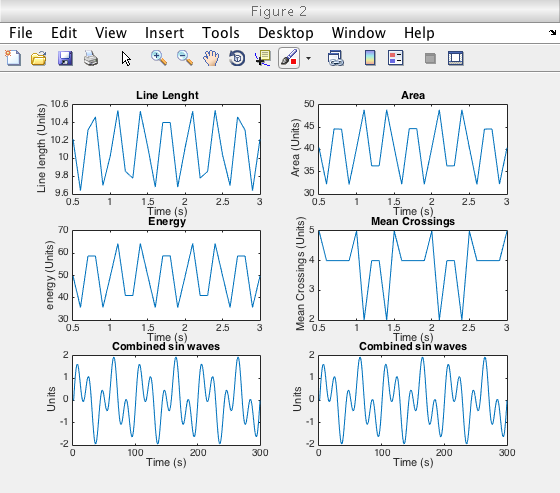
\includegraphics [width=4in]{BE521HW3_mlautman_02.png}
\begin{par}

\subsection*{2.1}

\end{par}
\begin{lstlisting}
dataset = 'I521_A0003_D001';
me = 'mlautman';
pass_file = 'mla_ieeglogin.bin';
[T,session] = evalc('IEEGSession(dataset, me, pass_file)');
data=session.data;
sample_rate = data.sampleRate ;
durration = data.channels(1).get_tsdetails.getDuration;
vals = session.data(1).getvalues(1:976078,1);

ms = floor(mod(durration/1e3,1000));
s = floor(mod(durration/1e6,60));
m = floor(mod(durration/1e6,3600)/60);
h = floor(mod(durration/1e6,3600*24)/3600);

mmss = num2str(ms);
ss = num2str(s);
mm = num2str(m);
hh = num2str(h);
[hh ':' mm ':' ss ':' mmss ' HH:MM:SS:MS']

msec = durration
time = '1:21:20:390' % from the IEEG explorer.
\end{lstlisting}

\color{lightgray} \begin{lstlisting}
ans =

1:21:20:390 HH:MM:SS:MS


msec =

     4.880390000000000e+09


time =

1:21:20:390

\end{lstlisting} \color{black}
\begin{par}

\subsection*{2.2}

\end{par}
\begin{lstlisting}
e = (h*3600 + m*60 + s)*sample_rate
vals = vals(1:e);
\end{lstlisting}

\color{lightgray} \begin{lstlisting}
e =

      976000

\end{lstlisting} \color{black}
\begin{par}

\subsection*{2.3a}

\end{par}
\begin{lstlisting}
zoInterp = @(x, numInterp) reshape(repmat(x,numInterp,1),1,[]);
\end{lstlisting}
\begin{par}

\subsection*{2.3b}

\end{par}
\begin{lstlisting}
figure(3)
plot(zoInterp(1:5,10), '-o')
title('ZoInterp');
\end{lstlisting}


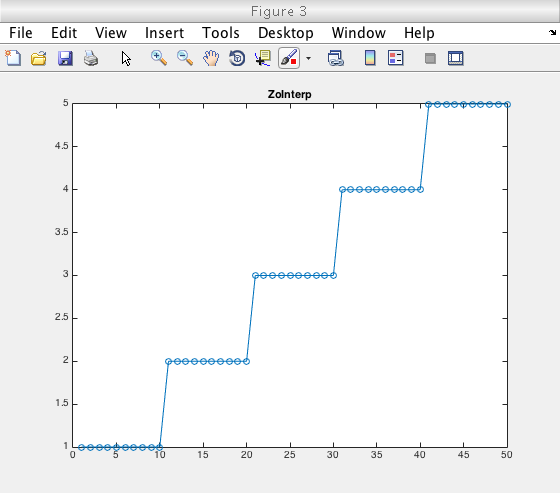
\includegraphics [width=4in]{BE521HW3_mlautman_03.png}
\begin{par}

\subsection*{2.4}

\end{par}



\end{document}
    
